\documentclass{standalone}
\usepackage{graphicx}	
\usepackage{amssymb, amsmath, amsthm}
\usepackage{color}

\usepackage{tikz}
\usetikzlibrary{intersections, backgrounds, math}

\definecolor{light}{RGB}{220, 188, 188}
\definecolor{mid}{RGB}{185, 124, 124}
\definecolor{dark}{RGB}{143, 39, 39}
\definecolor{highlight}{RGB}{180, 31, 180}
\definecolor{darkteal}{RGB}{29, 79, 79}
\definecolor{darkolive}{RGB}{97, 123, 45}
\definecolor{gray10}{gray}{0.1}
\definecolor{gray20}{gray}{0.2}
\definecolor{gray30}{gray}{0.3}
\definecolor{gray40}{gray}{0.4}
\definecolor{gray60}{gray}{0.6}
\definecolor{gray70}{gray}{0.7}
\definecolor{gray80}{gray}{0.8}
\definecolor{gray90}{gray}{0.9}
\definecolor{gray95}{gray}{0.95}

\tikzmath{
  function h(\x) {
    return 1.3 - 0.25 * \x - 0.5 * 9.806 * \x * \x;
  };
}

\begin{document}

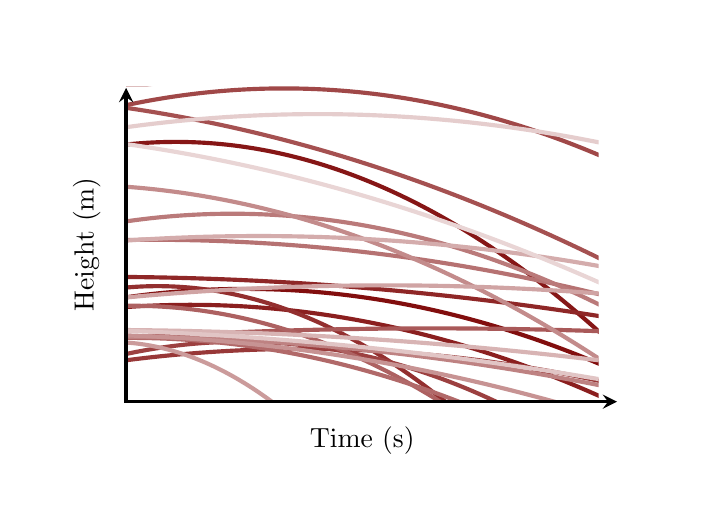
\begin{tikzpicture}[scale=1.0]
  
  \fill[white] (-4.25, -3) rectangle (4.25, 2.75);

  \begin{scope}
    \clip (-3, -2) rectangle (3, 2);
      
    \foreach \h/\v/\g [count=\n] in {0.663/0.636/3.801, 1.633/0.474/6.757, 0.601/0.313/3.471, 0.792/-0.039/0.998, 0.725/0.394/8.899, 0.263/0.579/2.322, 0.303/0.959/5.896, 1.883/0.954/4.283, 1.866/-0.656/2.319, 0.405/0.280/0.647, 0.609/0.055/6.446, 0.405/0.023/3.771, 1.027/0.063/1.736, 1.145/0.647/4.310, 0.413/-0.036/1.275, 1.365/-0.334/3.903, 0.421/-0.150/1.810, 0.376/-0.325/14.614, 0.662/0.419/1.143, 1.023/0.309/1.652, 0.455/-0.036/0.756, 1.991/0.747/1.131, 0.450/-0.160/0.898, 1.743/0.616/2.280, 1.636/-0.642/2.021} {
    \pgfmathsetmacro{\prop}{(100/ 26) * (30 - \n)};
    \colorlet{custom}{dark!\prop!white};
    \draw[domain={0:0.75}, smooth, samples=50, line width=1.5, variable=\t, color=custom] 
      plot ({9 * \t - 3}, { 2 * (\h + \v * \t - 0.5 * \g * \t * \t) - 2});
    }
    \fill[white] (-3, 2) rectangle (-2.7, 1.9);
  \end{scope}
  
  \draw [->, >=stealth, line width=1.25] (-3.00, -2.015) -- +(0, 4);
  \draw [->, >=stealth, line width=1.25] (-3.015, -2.00) -- +(6.25, 0);
  
  \node[rotate=90] at (-3.5, 0) { Height (m) };
  \node at (0, -2.5)  { Time (s) };
  
\end{tikzpicture}

\end{document}  
 